\documentclass[12pt,letterpaper, onecolumn]{exam}
\usepackage{amsmath}
\usepackage{amssymb}
\usepackage[lmargin=71pt, tmargin=1.2in]{geometry}
\usepackage{xcolor}
\usepackage[brazil]{babel}
\usepackage{natbib}
\usepackage{enumitem}
\usepackage{booktabs}
\usepackage[hidelinks]{hyperref}
\usepackage{graphicx}
\urlstyle{same}

\renewenvironment{solution}
{\par\noindent\textbf{R:}\enspace\color{blue}}
{\par\color{black}}

\thispagestyle{empty}

\begin{document}

\begingroup
\centering
\LARGE Lista 7 Gabarito - Econometria I - 2026\\[0.5em]
\large Prof: Andre Luiz Pereira Mancha \par
\large Monitor: Tuffy Licciardi Issa \par
\endgroup
\rule{\textwidth}{0.4pt}
\pointsdroppedatright
\printanswers
\renewcommand{\solutiontitle}{\noindent\textbf{Ans:}\enspace}
\newcommand{\qstar}{\hspace{-0.6em}\textsuperscript{*}\hspace{0.2em}}

\begin{questions}

\question (6.7, \citep{wooldridge2016}). As tres seguintes equacoes foram estimadas utilizando-se as 1.534 observacoes contidas no arquivo \texttt{401K}.

\[
\widehat{prate} = 80{,}29 + 5{,}44\,mrate + 0{,}269\,age - 0{,}00013\,totemp
\]
\[
(0{,}78)\qquad (0{,}52)\qquad (0{,}045)\qquad (0{,}00004)
\]
\[
R^2 = 0{,}100, \bar{R^2} = 0,098
\]

\[
\widehat{prate} = 97{,}32 + 5{,}02\,mrate + 0{,}314\,age - 2{,}66\,\log(totemp)
\]
\[
(1{,}95)\qquad (0{,}51)\qquad (0{,}044)\qquad (0{,}28)
\]
\[
R^2 = 0{,}144, \bar{R^2} = 0,142
\]

\[
\widehat{prate} = 80{,}62 + 5{,}34\,mrate + 0{,}290\,age - 0{,}00043\,totemp
\]
\[
(0{,}78)\qquad (0{,}52)\qquad (0{,}045)\qquad (0{,}00009)
\]
\[
\hspace{2.7cm} +\; 0{,}0000000039\,totemp^2
\]
\[
\hspace{2.7cm} \qquad (0{,}00000000010)
\]
\[
R^2 = 0{,}108, \bar{R^2} = 0,106
\]

Qual desses tres modelos voce prefere? Por que?

\begin{solution}
A \textbf{segunda especificacao} é preferível. Ela tem o maior \(R^2\) ajustado (\(0{,}142\)), e o uso de \(\log(totemp)\) parece mais razoável economicamente, pois permite um efeito marginal decrescente do tamanho da firma sobre a taxa de participação.
Assim, pela combinação de \textbf{melhor ajuste}, \textbf{parcimônia} e \textbf{interpretação econômica mais plausível}, a segunda equação e a melhor escolha.
\end{solution}

\vspace{0.7cm}

\question\qstar (6.10, \citep{wooldridge2016}). As duas equações seguintes foram estimadas usando dados do arquivo \texttt{MEAPSINGLE}. A principal variável explicativa e \texttt{lexppp}, o log dos gastos por estudante em nível escolar.

\[
\widehat{math4} = 24{,}49 + 9{,}01\,lexppp - 0{,}422\,free - 0{,}752\,lmedinc - 0{,}274\,pctsgle
\]
\[
(59{,}24)\qquad (4{,}04)\qquad (0{,}071)\qquad (5{,}358)\qquad (0{,}161)
\]
\[
n = 229,\quad R^2 = 0{,}472,\quad \bar{R}^2 = 0{,}462.
\]

\[
\widehat{math4} = 149{,}38 + 1{,}93\,lexppp - 0{,}060\,free - 10{,}78\,lmedinc - 0{,}397\,pctsgle + 0{,}667\,read4
\]
\[
(41{,}70)\qquad (2{,}82)\qquad (0{,}054)\qquad (3{,}76)\qquad (0{,}111)\qquad (0{,}042)
\]
\[
n = 229,\quad R^2 = 0{,}749,\quad \bar{R}^2 = 0{,}743.
\]

\begin{enumerate}[label=(\roman*)]
    \item Se você for um gestor de politicas publicas tentando estimar o efeito causal dos gastos por estudante sobre o desempenho na prova de matemática, explique por que a primeira equação e mais relevante do que a segunda. Qual e o efeito estimado de um aumento de 10\% nos gastos por estudante?

    \item A adição de \texttt{read4} a regressão tem efeitos estranhos sobre os coeficientes e significância alem de \(\beta_{lexppp}\)?

    \item De que forma você explicaria a alguém com apenas um conhecimento básico de regressões por que, neste caso, você preferiria a equação com o menor \(R\)-quadrado ajustado?
\end{enumerate}

\begin{solution}
\begin{enumerate}[label=(\roman*)]
    \item A primeira equação e mais relevante para inferência causal porque \texttt{read4} e uma variável de desempenho escolar muito próxima de \texttt{math4}. Ao inclui-la, parte do efeito dos gastos sobre matemática pode ser ``absorvida'' por uma variável que também reflete desempenho educacional. Em um modelo nivel-log, um aumento de 10\% em \texttt{lexppp} eleva \(math4\) em aproximadamente
    \[
    9{,}01 \times 0{,}10 = 0{,}901
    \]
    ponto percentual.

    \item Sim. O coeficiente de \texttt{lexppp} cai de \(9{,}01\) para \(1{,}93\) e perde significância estatística. O coeficiente de \texttt{free} também cai bastante em magnitude. Ja \texttt{lmedinc} fica muito mais negativo e passa a parecer estatisticamente importante, enquanto \texttt{pctsgle} aumenta em magnitude e também ganha significância. Isso sugere forte correlação de \texttt{read4} com as demais variáveis e que ela esta capturando grande parte da variação comum no desempenho escolar.

    \item \textbf{Um \(R^2\) maior não significa automaticamente um modelo melhor para causalidade}. A segunda equação prediz melhor porque usa uma variável muito próxima do próprio desempenho em matemática, mas isso não a torna mais útil para medir o efeito causal dos gastos. Se o objetivo é estimar esse efeito, a primeira equação e preferível, mesmo com menor \(R^2\) ajustado.
\end{enumerate}
\end{solution}

\vspace{0.7cm}

\question (6.3, \citep{wooldridge2016}) Utilizando os dados contidos no arquivo \texttt{RDCHEM}, a seguinte equacao foi obtida por MQO:

\[
\widehat{rdintens} = 2{,}613 + 0{,}00030\,sales - 0{,}0000000070\,sales^2
\]
\[
(0{,}429)\qquad (0{,}00014)\qquad (0{,}0000000037)
\]
\[
n = 32,\; R^2 = 0{,}1484.
\]

\begin{enumerate}[label=(\roman*)]
    \item Em que ponto o efeito marginal de \texttt{sales} sobre \texttt{rdintens} se torna negativo?
    \item Você manteria o termo quadrático no modelo? Explique.
    \item Defina \texttt{salesbil} como vendas expressas em bilhões de dólares: \(salesbil = sales/1.000\). Reescreva a equação com \texttt{salesbil} e \(salesbil^2\) como as variáveis independentes. Certifique-se de descrever os erros padrão e o \(R\)-quadrado. [Dica: Observe que \(salesbil^2 = sales^2/(1.000)^2\).]
    \item Com o proposito de reportar os resultados, qual equação você prefere?
\end{enumerate}

\begin{solution}
\begin{enumerate}[label=(\roman*)]
    \item O efeito marginal e
    \[
    \frac{\partial \widehat{rdintens}}{\partial sales}
    =
    0{,}00030 - 2(0{,}0000000070)\,sales.
    \]
    Igualando a zero,
    \[
    0{,}00030 = 0{,}000000014\,sales
    \]
    e portanto
    \[
    sales \approx 21428{,}57.
    \]
    Como \texttt{sales} esta em milhões de dólares, isso corresponde a cerca de \(21{,}43\) bilhões de dólares.

    \item O termo quadrático tem estatística t de aproximadamente
    \[
    \frac{-0{,}0000000070}{0{,}0000000037}\approx -1{,}89.
    \]
    Assim, ele não e claramente significante a 5\%, embora haja alguma evidencia de curvatura a 10\%. Eu o manteria apenas se quisesse permitir explicitamente retornos decrescentes; caso contrario, ha argumento para um modelo mais simples.

    \item Como \(sales = 1000\,salesbil\) e \(sales^2 = 1000000\,salesbil^2\), a equação fica
    \[
    \widehat{rdintens} = 2{,}613 + 0{,}30\,salesbil - 0{,}0070\,salesbil^2.
    \]
    Os erros padrão também mudam de escala:
    \[
    (0{,}429)\qquad (0{,}14)\qquad (0{,}0037).
    \]
    O \(R^2\) permanece
    \[
    R^2 = 0{,}1484.
    \]

    \item Para reportar os resultados, eu prefiro a equação com \texttt{salesbil}, pois os coeficientes ficam muito mais legíveis e fáceis de interpretar, sem alterar ajuste, sinais ou significância.
\end{enumerate}
\end{solution}

\vspace{0.7cm}

\question\qstar (5.5, \citep{wooldridge2016}) O histograma a seguir foi criado usando-se a variável \textit{score} do arquivo \texttt{ECONMATH}. Foram usadas trinta divisões para cria-lo, e a altura de cada célula e a proporção de observações dentro do intervalo correspondente. A distribuição normal de melhor ajuste isto é, usando a media amostral e o desvio padrão amostral  foi sobreposta no histograma.

\begin{center}
    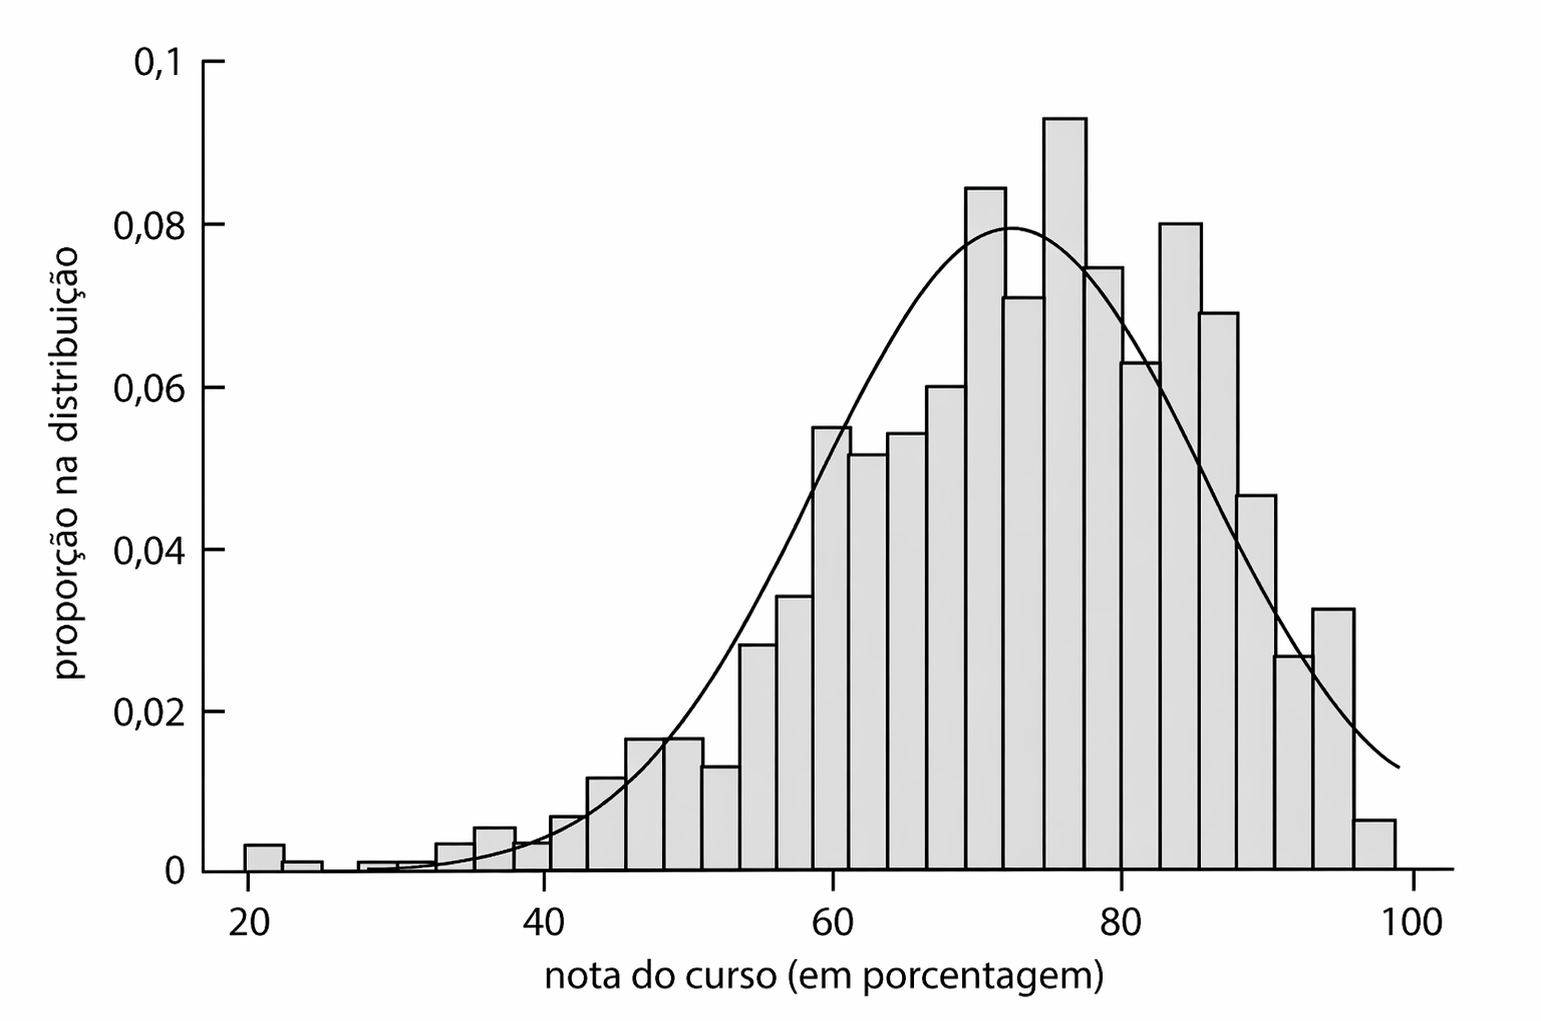
\includegraphics[width=0.75\textwidth]{graph.png}
\end{center}

\begin{enumerate}[label=(\roman*)]
    \item Se você usar a distribuição normal para estimar a probabilidade de \textit{score} superar 100, a resposta seria zero? Por que sua resposta contradiz a hipótese de uma distribuição normal de \textit{score}?

    \item Explique o que esta acontecendo na parte esquerda do histograma. A distribuição normal se ajusta bem a parte esquerda do gráfico?
\end{enumerate}

\begin{solution}
\begin{enumerate}[label=(\roman*)]
    \item Não. Se \textit{score} fosse exatamente normal, haveria sempre probabilidade positiva de observar valores acima de 100, porque a distribuição normal tem suporte em toda a reta real. Isso contradiz o fato de que notas em porcentagem são naturalmente limitadas superiormente por 100.

    \item A distribuição apresenta \textbf{assimetria a esquerda}: a maior parte das notas esta entre 60 e 90, mas existe uma cauda mais longa de notas baixas. Na parte esquerda do histograma, vemos mais massa em valores baixos do que uma normal ajustada sugeriria. Portanto, a normal não se ajusta tao bem a cauda esquerda.
\end{enumerate}
\end{solution}

\question\qstar (6.C9, \citep{wooldridge2016})\footnote{Esta e uma questão computacional. Para instalar o \texttt{R} e o \texttt{RStudio} veja o passo a passo aqui: \href{https://rstudio-education.github.io/hopr/starting.html}{https://rstudio-education.github.io/hopr/starting.html}. Caso tenha duvidas quanto a linguagem, consulte o material disponibilizado no Moodle, e recomendo também o seguinte material de introdução ao \texttt{R}: \href{https://fhnishida.netlify.app/project/rec2301/sec2/}{https://fhnishida.netlify.app/project/rec2301/sec2/} }. O conjunto de dados \texttt{NBASAL} contem informacoes salariais e estatisticas carreira de 269 jogadores da National Basketball Association (NBA).

\begin{enumerate}[label=(\roman*)]
    \item Estime um modelo que relacione pontos por jogo (\textit{points}) aos anos na liga (\textit{exper}), \textit{age} e \textit{years} jogando na universidade (\textit{coll}). Inclua um termo quadrático em \textit{exper}; as outras variáveis devem aparecer em nível. Registre os resultados na forma usual.

    \item Mantendo os anos na universidade e a idade fixos, por qual valor de experiencia o ano seguinte de experiencia reduziria os pontos por jogo? Isso faz sentido?

    \item Por que você acha que \textit{coll} tem um coeficiente negativo e estatisticamente significativo? (Dica: Jogadores da NBA podem ser convocados antes de terminar suas carreiras universitárias e ate mesmo diretamente do Ensino Médio.)

    \item Adicione um termo quadrático em \textit{age} a equação. Ele e necessário? O que isso parece sugerir em relação aos efeitos de idade, uma vez que experiencia e educação estão controladas?

    \item Agora faca a regressão de log(\texttt{wage}) sobre \texttt{points}, \texttt{exper}, \texttt{exper$^2$}, \texttt{age} e \texttt{coll}. Relate os resultados de forma usual.

    \item Teste se \texttt{age} e \texttt{coll} são conjuntamente significativos na regressão do item (v). O que isso implica em relação a idade e educação terem efeitos separados sobre salario, uma vez que produtividade e tempo de serviço são levados em conta?
\end{enumerate}

\end{questions}
\bibliographystyle{apalike}
\bibliography{refs}
\end{document}
